\chapter{Introduction}
\label{chap:intro}

In the early 1990s it was suggested that linguistics might be the first academic discipline to preside over its own demise. As much as 90\% of the world’s 7,000 languages were predicted to become extinct by the end of the 21st century \citep{krauss_worlds_1992,krauss_keynote--mass_2007,campbell_new_2013}. 
Linguists responded by putting greater emphasis on the documentation and description of endangered languages, and over the past thirty years have steadily broadened our knowledge of the world's languages. Today the estimate has been reduced \cite{eberhard_ethnologue:2020} but we still have little data or knowledge about most of the endangered languages. It is critical that languages be documented and described quickly before they disappear. % without sufficient accessible data.Since the disquieting warning about language endangerment, 
%Linguistic structures and language development cannot be studied without accessible data. 
%We have little data or knowledge about most of those languages, making it critical to document and describe new languages quickly. 

\begin{figure}[tb]
\centering
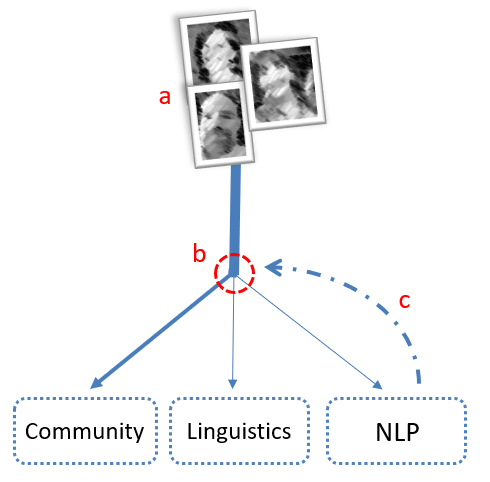
\includegraphics[width=5.75cm]{figs/Flowchart.PNG}
\caption[Language Data Production]{Language Data Production}
\label{fig:flowchart}
\end{figure}

The general flow of documentary and descriptive work is illustrated in Figure \ref{fig:flowchart}. A team of linguists and native speakers (a) collaborate to document and conduct basic linguistic analysis and annotate language data. Annotated data can be used for linguistic research, NLP development, and to benefit the community of speakers. However, because annotation is time- and labor-intensive work, a significant portion of documented language data remains inaccessible (b) to the first two groups, and to a lesser extent, to the communities. The methods presented here will make more data accessible by integrating NLP machine learning systems to speed and improve linguistic analysis and annotation (c). The research also looks at ways linguists and NLP scientists may want to adjust their expectations and customary workflows in order to more effectively integrate machine learning and linguistic field data for optimal results. 

Current methods in language documentation and description are
%including the process of annotating texts and analyzing morphological paradigms, 
are too slow to counteract the crisis of language endangerment.
If the production of accessible data is to match the pace of language extinction, computational methods must be effectively integrated into the workflow of language documentation and description. However, natural language processing (NLP) has not responded as quickly to the language endangerement crisis. Since the 1990s, machine learning systems, capable of learning complex patterns in data, have gained tremendous success in NLP
%Typically, state-of-the-art systems, specifically neural networks, require hundreds of thousands, or even millions, of data instances (words, sounds, sentences, etc.) to achieve state-of-the-art results. Few languages have more than a couple of thousand tokens,
%, let alone much available data, 
but research has been focused on a handful of beyond a handful economically or politically powerful languages such as Chinese, Arabic, English and other European languages. These languages are well documented and described. None 
%demonstrate complicated morphology polysynthetic type, none are under-documented, none 
are endangered.%\mans{The big data requirement is pretty specific to neural models.} 

Fortunately, this is changing. In recent years, NLP research with limited data has burgeoned. This is evidenced, for instance, by the 2015-2019 DARPA-funded LORELEI project, motivated in part by the 2014 Haiti earthquake where disaster aid was hampered by language. Haitian Creole is a language rarely encountered in NLP. When medicine and clean water were available, foreign aid workers struggled to process information that told them where supplies were most urgent. 

Despite this growth, very few NLP systems have been integrated into the process of documenting and describing endangered languages. This is undoubtedly due in large part to the fact that state-of-the-art supervised machine learning models depends on large amounts of annotated data (on the order of hundreds of thousands or millions of tokens) and to challenges presented by the dynamic, evolving nature of ongoing linguistic analysis and the inconsistencies that arise from manual annotation of field data. To overcome these challenges methods must be developed that allow documentary and descriptive linguists from NLP and \textit{vice versa}.
This dissertation investigates methods for more effectively leveraging machine learning systems for language documentation and description, particularly for morphological analysis and annotation. 


%\section{Overview of Research}

This work is motivated by a “yawning gap” between the amount of documented data deposited in language archives and the portion of the data that is actually usable for research \citep{seifart_language_2018}. This gap is caused by what has been described as an ``annotation bottleneck'' (Figure \ref{fig:bottleneck}) because currently tedious, time-consuming, and expensive annotations are performed primarily by hand from start to finish \citep{simons_worlds_2013,holton_developing_2017}. Manual annotation is subject to human error, introducing inconsistencies and typos, due often not to the difficulty of the task, but to its repetitive and monotonous nature. Other noise in the annotation arise because early annotation is the method for linguists to discover and understand the language's structure. As their understanding grows, analyses change and this is reflected in later annotations.
Budget and time constraints often mean that large portions of the data produced by field projects are left uncorrected and simply unannotated. The unannotated portions of documentary corpora remain untapped resources. 
%These resources could inform the development of linguistics science and NLP. They could also build human language technology that would benefit the communities that speak them. 

The overarching question of this dissertation asks: \emph{How might the integration of machine learning into language documentation and description affect currently accepted expectations, methods, and workflows?} It addresses that question by examining how current expectations and methods affect machine learning performance on morphological analysis and annotation and exploring new methods for effectively exploiting existing annotations to boost machine learning performance on these tasks. This will be done with three studies with various NLP machine learning models and documentary and descriptive corpora from several under-documented languages:

\begin{figure}[t]
    \centering
    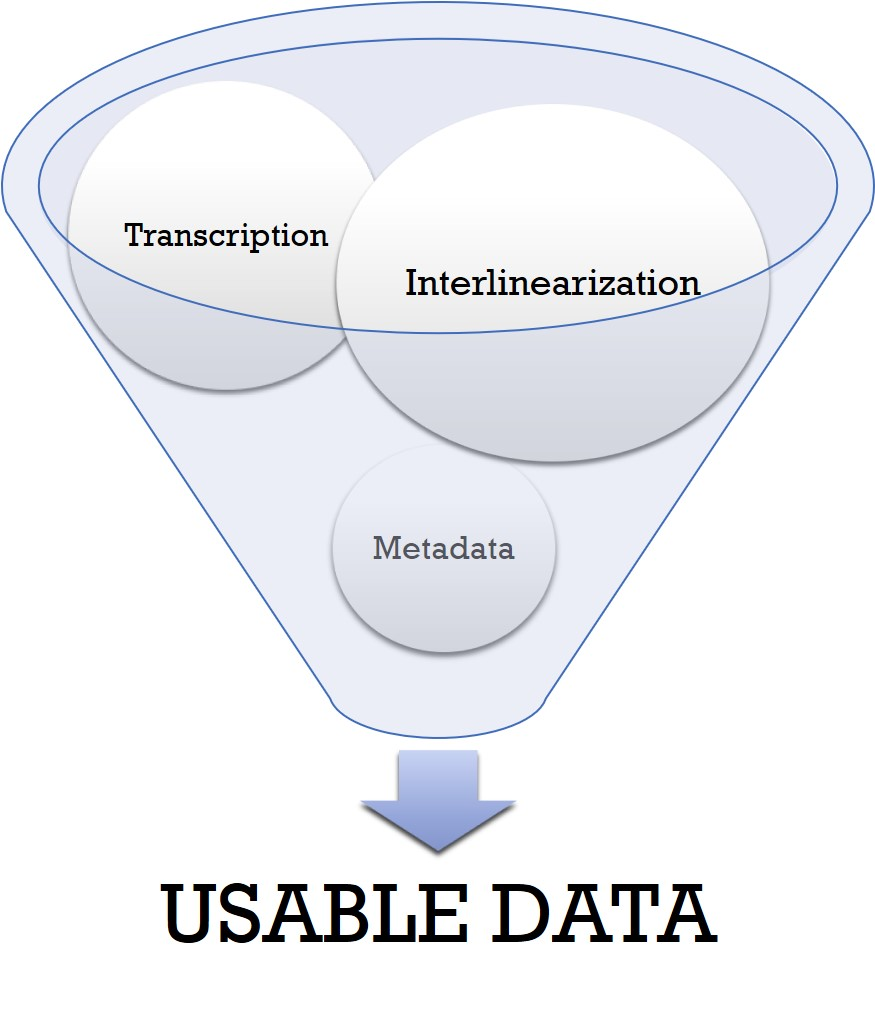
\includegraphics[width=5.5cm]{figs/AnnotationFunnel.jpg}
    \caption[Annotation Bottleneck]{Annotation bottleneck in language documentation and description.}
    \label{fig:bottleneck}
\end{figure}


\begin{enumerate}
\item{} \emph{Automating Segmentation and Glossing:} How do variations conventional expectations from NLP and from linguistics and their resulting research designs affect machine learning performance on morpheme segmentation and glossing of documentary and descriptive data? 

\item{} \emph{Morphological Paradigm Induction from Interlinear Glossed Texts (IGT2P):} To what extent can machine learning models learn morphological inflection patterns from manually interlinearized texts?

\item \emph{Priority of Part of Speech Tagging:} 
What impact does traditional high priority of part of speech tagging in NLP have on machine learning of morpheme segmentation and glossing and paradigm induction?
\end{enumerate}


%\section{Contributions}

The goals of this research is four-fold. First, it shows that it is possible and practical to use machine learning to perform annotation by developing and applying methods that improve results on typologically diverse languages with limited training data. Second, by learning inflectional paradigms and accurately generation inflected forms, it demonstrates that machine learning can be used to build and test hypotheses about a language's morphological structure. Third, by training on noisy linguistic field data rather than curated and polished data that NLP systems are typically trained on, this research proves that the sometimes only annotated data available for a under-documented language can be used to effectively train machine learning models. 
%As such, it may uncover as-yet unforeseen challenges for NLP systems in low-resource settings. 
%It will study what happens when NLP priorities are borrowed directly for documentary and descriptive linguistics, specifically the priority of part of speech (POS) tagging. 
Fourth,  it will increases annotated data in several low-resource languages that represent a range of linguistic structures and language families. This increased annotated data allows more thorough testing of linguistic theories and computational models.
In summary, this work will establish that new computational methods can be successfully integrated into language documentation and description. 

%One goal of the research is to prove that machine learning systems can achieve reasonable performance when trained on the often noisy data produced by documentary and descriptive projects.

%study effective integration of computational methods that could open the annotation bottleneck. 
%caused by current time-consuming manual methods to produce morpheme segmentation, glossing, free translation, and first-pass hypotheses of morphological inflectional paradigms. 

%First, with successful automated joint segmentation and glossing it will integrate machine learning into the documentary and descriptive pipeline for several typologically different languages. This will demonstrate the potential for producing new annotated data more quickly and accurately than is possible with current methods. While other research has demonstrate this with systems for one or two languages, this research will be conducted on several languages and will show the practicality of automated assistance for morphological annotation regardless of language typology. 

%Second, by testing a process to learn inflectional paradigms from field data the proposed dissertation will demonstrate the potential for machine learning to assist linguists in deeper analysis and description. This is a step towards integrating machine learning assistance beyond early documentary stages and using it to build and test holistic hypotheses about a language's structure.

%Third, the dissertation will unite the efforts of linguistics and NLP by successfully training machine learning on linguistic field data. A main theme of the proposed research is that machine learning systems can achieve reasonable performance when trained on the often noisy output produced by documentary and descriptive projects. Rather than the curated published data that NLP systems are normally trained on, this research will leverage interlinearized glossed texts from documentary and descriptive field work. Since this research will be performed on ``real live” field data---sometimes the only annotated data available for a language---it may uncover as-yet unforeseen challenges for NLP systems in low-resource settings.
%Specifically, it will use neural networks to learn inflectional patterns in five languages.
%\mans{``neural machine learning'' is perhaps a little too loose: neural networks might be better.}

%Third, it will establish not only that new computational methods can be successfully integrated into language documentation and description, but it will show how linguistics field methods may impact NLP systems and test whether certain NLP assumptions about data annotation should impact linguistics field methods. It will do this by studying what happens when NLP priorities are borrowed for documentary and descriptive linguistics, specifically the priority of part of speech (POS) tagging. Additionally, the discussions of other studies will focus on the characteristics and quality of the manually annotated data and how these characteristics affect the machine learning's performance.

%Fourth, the proposed research will increase annotated data in five low-resource languages. These languages represent a range of linguistic structures and language families. They are spoken by communities across five continents. Interlinear texts in these languages are currently limited to 5-100K words and the amount of descriptive publications is quite low. Increased annotated data will allow more thorough testing of linguistic theories and computational models.
%, which contribute to our understanding of human language and the performance of machine learning algorithms in low-resource settings. 

%\section{Organization of Prospectus}

%This Prospectus describes the author's planned dissertation research. Chapter \ref{chap:litreview} reviews issues in previous research that are related to the proposed research. Chapter \ref{chap:datamodels} describes the data and computational models the research will use. 